\documentclass[10pt,letterpaper]{article}
\usepackage[spanish]{babel}
\usepackage{listings}
\usepackage{blindtext} 
\usepackage{graphicx}
\usepackage{float}
\usepackage{xcolor}

% Preámbulo
\title{Sistema de gestión de una Biblioteca Universitaria}
\author{Sergio De Luis}
\date{\today}

\definecolor{codegreen}{rgb}{0,0.6,0}
\definecolor{codegray}{rgb}{0.5,0.5,0.5}
\definecolor{codepurple}{rgb}{0.58,0,0.82}
\definecolor{backcolour}{rgb}{0.95,0.95,0.92}

\lstdefinestyle{mystyle}{
    backgroundcolor=\color{backcolour},   
    commentstyle=\color{codegreen},
    keywordstyle=\color{magenta},
    numberstyle=\tiny\color{codegray},
    stringstyle=\color{codepurple},
    basicstyle=\ttfamily\footnotesize,
    breakatwhitespace=false,         
    breaklines=true,                 
    captionpos=b,                    
    keepspaces=true,                 
    numbers=left,                    
    numbersep=5pt,                  
    showspaces=false,                
    showstringspaces=false,
    showtabs=false,                  
    tabsize=2
}
\lstset{style=mystyle}

\renewcommand{\lstlistingname}{Código}
\renewcommand{\lstlistlistingname}{Lista de códigos}

\begin{document}

\maketitle

\tableofcontents
\newpage 
\lstlistoflistings
\listoffigures
\newpage

\section{Introducción}

\section{Descripción del problema}
Una biblioteca universitaria necesita digitalizar su operación. Actualmente lleva el control en papel y requiere un sistema computacional que gestione su acervo, los préstamos y los usuarios.

\subsection{Análisis y diseño}
La biblioteca cuenta con \textbf{libros}, de los cuales puede tener varios \textbf{ejemplares} físicos para cada título. Cada libro tiene un título, año de publicación, ISBN y pertenece a una o más \textbf{categorías} (Ciencias, Humanidades, Ingeniería, etc.). Además, cada libro fue escrito por uno o más \textbf{autores}.

Los \textbf{usuarios} pueden ser estudiantes o profesores. De cada uno se guarda el nombre, correo, número de cuenta y tipo. Un usuario puede tener \textbf{activos} varios préstamos simultáneos (máximo 3), pero un ejemplar solo puede estar prestado a un usuario a la vez.

Cada \textbf{préstamo} registra la fecha de salida, la fecha de devolución esperada, y la fecha real de devolución (en el caso en el que ya se haya devuelto el ejemplar). Si un préstamo se devuelve más tarde, se registra una \textbf{multa} con el monto y si fue pagada o no.

\subsection{Modelo Entidad-Relación}
\begin{figure}[H]
    \centering
    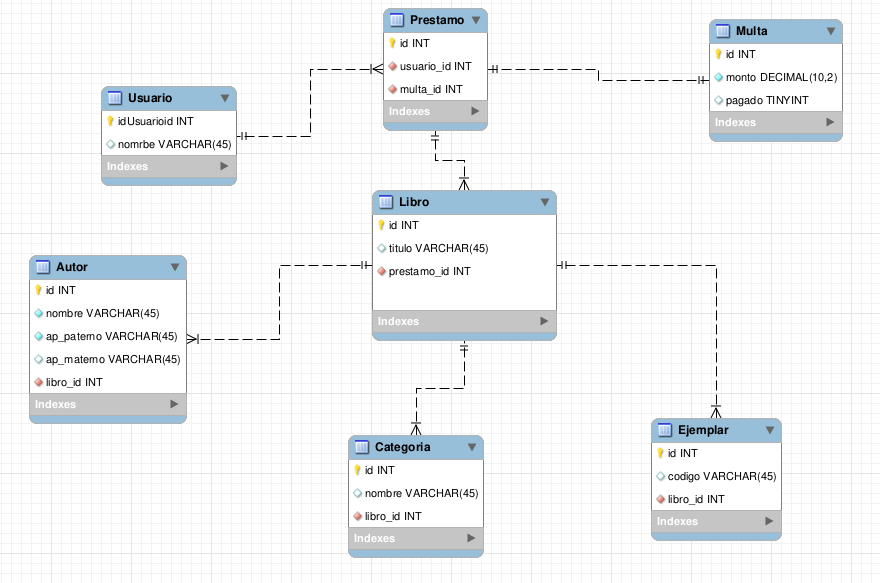
\includegraphics[width=0.8\textwidth]{mer.png}
    \caption{Modelo ER para el sistema de gestión de biblioteca}
\end{figure}

\subsection{Implementación y validación}

% Se añade 'inputencoding=latin1' para digerir los acentos del archivo SQL antiguo
\lstinputlisting[language=SQL, frame=single, numbers=left, inputencoding=latin1, caption={Script de creación de las tablas para el modelo de datos}]{codes/create.sql}

% Se añade 'inputencoding=latin1' para digerir los acentos del archivo SQL antiguo
\lstinputlisting[language=SQL, frame=single, numbers=left, inputencoding=latin1, caption={Script de inserción de datos sobre la estructura del modelo de datos}]{codes/insertions.sql}

\section{Conclusiones}

\section{Bibliografía}

\end{document}